\chapter{Einleitung}
Quantenstrukturen, wie sie heutzutage hergestellt werden können, eröffnen neue Möglichkeiten im Bereich der ultraschnellen Elektronik und Photonik. Solche Strukturen lassen sich in aller Regel als \emph{offene} Systeme beschreiben. Es findet ein Austausch von lokal erhaltenen Fermionen -- die Erhaltung wird durch eine lokale Kontinuitätsgleichung beschrieben -- mit der Umgebung statt. Die Umgebung besteht dabei aus mindestens zwei verschiedenen Teilchen-Reservoirs. In diesem Fall kann also ein Nicht-Gleichgewichtszustand erreicht werden, beispielsweise durch das Anlegen einer Spannung. Das zu untersuchende System besitzt eine endliche Ausdehnung im Raum. Es muss im Nicht-Gleichgewichtsfall folglich ein Strom durch die Oberfläche als Rand des Systems fließen. Wir beschränken uns hier auf eindimensionale Quantenstrukturen, für die also die interessante Physik in einer Dimension stattfindet. Dabei wollen wir den Strom der Teilchen, also den quantenmechanischen Transport beschreiben. Dies geschieht allgemein in verschiedenen Anwendungsfällen (Hydrodynamik, Aerodynamik, Elektronik, Neutronentransport, \dots) mit Hilfe einer die Dynamik beschreibenden Differentialgleichung. Hierfür werden Randbedingungen benötigt. Eben diese Randbedingungen definieren den offenen (oder auch geschlossenen) Charakter des Systems.

\chapter{Entwicklung}

\section{Zum Dichteoperator}
\todo{Datta}
Wir konzentrieren uns im folgenden lediglich auf ein Modell unabhängiger Elektronen, sodass es genügt, den Einteilchen-Dichteoperator zu betrachten.

\section{Herleitung der Liouville-von-Neumann Gleichung}
Die Liouville-von-Neumann Gleichung erhält man aus der Liouville-Gleichung wie folgt.
\begin{align}
  \partial_t \hat{\rho} &= \frac{i}{\hbar}\left[\hat{\rho} , H\right] \\
  \underbrace{\bra{x} \partial_t \hat{\rho} \ket{y}}_{\equiv \partial_t \rho(x,y)} &= \bra{x}\ket{\frac{i}{\hbar}\left[\hat{\rho} , H\right]y} \\
   &= \frac{i}{\hbar} \sum_k p_k ( \underbrace{\bra{x}\ket{\Psi_k}}_{\equiv \Psi_k(x)}\bra{\Psi_k}\ket{Hy} - \bra{x}\ket{H\Psi_k}\underbrace{\bra{\Psi_k}\ket{y}}_{\equiv \Psi_k^*(y)} )
\end{align}
Mit dem Hamiltonoperator für ein einzelnes Teilchen in einer Dimension in Ortsdarstellung
\begin{align}
  \left[ -\frac{\hbar^2}{2m}\frac{\partial^2}{\partial x^2} + V(x) \right] \Psi(x) = \bra{x}\ket{H\Psi} \equiv \mathcal{L}(x)\Psi(x)
  \label{eq:Liouville-Operator}
\end{align}
folgt mit $H^{\dagger} = H$
\begin{align}
  \partial_t \rho(x,y) &= \frac{i}{\hbar} \sum_k p_k \left( \Psi_k(x)\mathcal{L}^*(y)\Psi_k^*(y) - \mathcal{L}(x)\Psi_k(x)\Psi_k^*(y) \right) \\
  &= \frac{i}{\hbar}  (\mathcal{L}^*(y) - \mathcal{L}(x)) \sum_k p_k \left( \Psi(x)\Psi^*(y) \right) \\
  &= \frac{i}{\hbar}  (\mathcal{L}^*(y) - \mathcal{L}(x)) \bra{x}\left(\sum_k p_k  \ket{\Psi_k}\bra{\Psi_k} \right)\ket{y} \\
  &= \frac{i}{\hbar}  (\mathcal{L}^*(y) - \mathcal{L}(x))\rho(x,y)
\end{align}
Wir definieren noch
\begin{align}
  \mathcal{L}(x,y) &\equiv \mathcal{L}(x) - \mathcal{L}^*(y)\\
   &= -\frac{\hbar^2}{2m}\left( \partial_x^2 - \partial_y^2 \right) + V(x) - V^*(y)
\end{align}
und erhalten die Liouville-von-Neumann Gleichung im Ortsraum
\begin{equation}
  \partial_t \rho(x,y) = \frac{1}{i\hbar} \mathcal{L}(x,y) \rho(x,y) \; .
  \label{eq:lvn_first}
\end{equation}
Es lassen sich zwei Fälle unterscheiden:
\begin{itemize}
  \item Der stationäre Fall mit $\partial_t \rho(x,y,t) = 0$
  \item der allgemeinere transiente Fall $\partial_t \rho(x,y,t) \neq 0$.
\end{itemize}

\section{Schwerpunkt- und Relativkoordinaten}
Wir führen die Schwerpunkt- und Relativkoordinaten
\begin{align}
  &r \equiv \frac{x+y}{2} \qquad &q \equiv x-y \label{eq:gedrehteKoordinaten}\\
  \Leftrightarrow\qquad &x = r+\frac{q}{2} \qquad &y = r-\frac{q}{2}
\end{align}
ein. Die Ableitungen transformieren sich dabei gemäß
\begin{align}
  \partial_r \partial_q  &= \partial_r \left( \frac{\partial}{\partial x} \frac{\partial x}{\partial q} + \frac{\partial}{\partial y} \frac{\partial y}{\partial q}\right) \\
   &= \left( \frac{\partial}{\partial x} \frac{\partial x}{\partial r} + \frac{\partial}{\partial y} \frac{\partial y}{\partial r}\right) \left( \frac{\partial}{\partial x} \frac{1}{2} + \frac{\partial}{\partial y} \frac{-1}{2}\right)\\
    &= \left( \frac{\partial}{\partial x} 1 + \frac{\partial}{\partial y} 1\right) \left( \frac{\partial}{\partial x} \frac{1}{2} + \frac{\partial}{\partial y} \frac{-1}{2}\right)\\
   &= \frac{1}{2}\partial_x \partial_x - \frac{1}{2}\partial_x \partial_y + \frac{1}{2}\partial_y \partial_x - \frac{1}{2}\partial_y \partial_y \\
  &=  \frac{1}{2}(\partial_x^2 - \partial_y^2) \; ,
\end{align}
wobei im letzten Schritt der Satz von Schwarz genutzt wird. Damit ergibt sich der transformierte Liouville Operator zu
\begin{align}
  \mathcal{L}(r,q) = -\frac{\hbar^2}{m} \partial_r\partial_q + \underbrace{V\left(r+\frac{q}{2}\right) - V^*\left(r-\frac{q}{2}\right)}_{\equiv \tilde{B}(r,q)}
\end{align}
Mit der Umbenennung
\begin{align*}
  \rho \longrightarrow u \\
  r \longrightarrow \tilde{x} \\
  q \longrightarrow \tilde{y} \\
  t \longrightarrow \tilde{t}
\end{align*}
lautet die LvN Gleichung nun
\begin{align}
  i\hbar\partial_{\tilde{t}} u(\tilde{x},\tilde{y})+\frac{\hbar^2}{m}\operatorname{div}(A\nabla u(\tilde{x},\tilde{y})) -  \tilde{B}(\tilde{x},\tilde{y}) u(\tilde{x},\tilde{y}) = 0
\end{align}

\section{Charakteristische Einheiten}
Zunächst wird die  \lvn in eine einheitenlose Form gebracht.
\begin{align}
    i\frac{\hbar}{V_0}\partial_{\tilde{t}}\, u(\tilde{x},\tilde{y})+\frac{\hbar^2}{mV_0}\operatorname{div}(A\nabla u(\tilde{x},\tilde{y})) - \frac{\tilde{B}(\tilde{x},\tilde{y})}{V_0} u(\tilde{x},\tilde{y}) = 0
\end{align}
Energien werden in Einheiten von $V_0$ gemessen, welche wir im weiteren Verlauf als die Potentialbarriere $V_0 = \SI{0.1768}{\electronvolt}$ wählen werden.

Wir führen folgende Skalierung ein, um nun auch Zeiten und Orte einheitenlos zu behandeln.
\begin{align}
  \left(\begin{array}{c}\tilde{x}\\\tilde{y}\end{array}\right) &= \xi \left(\begin{array}{c}x\\y\end{array}\right)   & \xi &= \sqrt{\frac{\hbar^2}{mV_0}} \\
  \tilde{t} &= \tau t   & \tau &= \frac{\hbar}{V_0}
\end{align}
Damit folgt
\begin{align}
  \partial_{\tilde{t}} &= \frac{\partial}{\partial (\tau t)} = \tau^{-1} \partial_t = \frac{V_0}{\hbar} \partial_t \\
  \partial_{\tilde{x}}^2 &= \frac{\partial^2}{(\partial (\xi x))^2} = \xi^{-2} \partial_x^2 = \frac{mV_0}{\hbar^2} \partial_x² \; ,
\end{align}
sodass die \lvn die Form
\begin{align}
  i \partial_t u(x,y)+\operatorname{div}(A\nabla u(x,y)) - B(x,y) u(x,y) = 0
  \label{eq:lvn}
\end{align}
annimmt. Hierbei ist
\begin{align}
  B(x,y) \equiv \frac{\tilde{B}(x,y)}{V_0} = \frac{V\left(x+\frac{y}{2}\right) - V^*\left(x-\frac{y}{2}\right)}{V_0}
\end{align}
eingeführt worden. Die Skalierung lässt sich berechnen, indem die effektive Masse als konstant
\begin{align}
  m = 0.063 m_0 =  0.063\cdot\SI{9.1e-31}{\kilogram}
\end{align}
angenommen wird. Damit ergibt sich folgende Skalierung zwischen SI-Einheiten und den hier eingeführten einheitenlosen Größen.
\begin{align}
  V_0 &= \SI{0.1768}{\electronvolt} \\
  \xi &= \SI{2.62e-9}{\meter}
 \\
  \tau &= \SI{3.72e-15}{\second}

\end{align}

\section{Randbedingungen}
Die Dynamik des in der Einleitung skizzierten Systems muss irreversibel in der Zeit sein. Andernfalls sind instabile Lösungen in der Zeit zulässig \cite{frensley2}. Solche instabilen Lösungen lassen sich anhand des Eigenwertspektrums des Liouvilleoperators aus Gleichung \eqref{eq:lvn_first} erkennen. Man kann zeigen, dass für geschlossene, konservative Systeme $\mathcal{L}$ hermitsch ist als Folge der Hermitizität des Hamiltonoperators $H$ \cite{frensley2}.
\begin{align}
  H- H^{\dagger} = \frac{\hbar}{i}\int_s \vb{j}\diff\vb{s} = 0
\end{align}
Der Nettostrom durch die Oberfläche ist also Null. Damit treten lediglich oszillierende Lösungen der \lvn auf. Da wir nun offene Systeme modellieren wollen, müssen wir das Ein- und Austreten von Teilchen in das System erlauben und verletzen dadurch die Hermitizität von $H$ und $\mathcal{L}$. Dadurch wird mindestens ein Eigenwert einen nicht-verschwindenden imaginären Teil bekommen. Anhand Gleichung \eqref{eq:lvn_first} sehen wir, dass in der Zeit instabile Lösungen für Eigenwerte mit positivem Realteil auftreten. Falls die Randbedingungen reversibel in der Zeit sind, so sind die Realteile der Eigenwerte symmetrisch und es existieren unphysikalische, instabile Lösungen \cite{frensley2}. Ein Beispiel hierfür ist $\partial \rho /\partial r = 0$ entlang $x=0$ und $y=0$. Diese Randbedingung ist insofern plausibel, da sie zu konstanter Dichte an den Rändern führt und damit den Effekt eines fixierten chemischen Potentials beschreibt. Sie führt jedoch wegen der Zeit-Umkehrbarkeit zu unphysikalisch exponentiell steigenden Lösungen.

Die Randbedingungen müssen also irreversibel in der Zeit sein und ferner die Stabilität des Systems sicherstellen. Ein hierfür geeigneter Ansatz wird erstmals in \cite{frensley2} getroffen, indem die Reservoire in Analogie zu einem schwarzen Körper gesehen werden. In das Reservoir eintretende Teilchen werden vollständig absorbiert. Umgekehrt "strahlt" das Reservoir Teilchen entsprechend der thermischen Gleichgewichts-Verteilung in das System ein. Damit ist klar, dass Randbedingungen für \emph{Inflow-}Teilchen mit positiver Geschwindigkeit am linken Rand und solche mit negativer Geschwindigkeit am rechten Rand gesetzt sind, während für \emph{Outflow}-Teilchen keine Randbedingung vorgegeben ist. Wir müssen also dazu in der Lage sein, Teilchen nach ihrer Geschwindigkeit zu unterscheiden.
Es ist daher ein natürliches Vorgehen, nach einer Wahrscheinlichkeitsverteilung im Phasenraum zu fragen. Dieser Frage ging Eugene Wigner 1932 nach \cite{wigner} und formulierte die nach ihm benannte Wignerverteilung $P(r, k)$, siehe Kapitel \ref{sec:wignerfunktion}. Die klassische Position eines Teilchens wird dann mit $r$ aus Gleichung \eqref{eq:gedrehteKoordinaten} und der klassische Impuls mit $p=\hbar k$ identifiziert.
Dabei ist $k$ die zu $q$ aus Gleichung \eqref{eq:gedrehteKoordinaten} gehörende Wellenzahl. Positive und negative Geschwindigkeiten lassen sich einfach durch das Vorzeichen von $k$ unterscheiden, sodass sich die Randbedingungen konkretisieren lassen.
\begin{align}
  P(-L/2,k)|_{k>0} &= f_l(k) \\
  P(+L/2,k)|_{k<0} &= f_r(k)
\end{align}
Die Gleichgewichts-Verteilung der Reservoire $f_{l,r}(k)$ ergibt sich aus der Fermi-Dirac-Statistik wie folgt.
\begin{align}
  \frac{\expval{N}}{A_{\perp}} &= 2\frac{1}{A_{\perp}}\sum_{\vb{k}}\frac{1}{1+\exp(\beta(\epsilon(\vb{k}) - \mu))} \\
    &= 2\frac{1}{A_{\perp}}  \frac{A_{\perp}}{(2\pi)^2} \sum_{k_z}\int_{-\infty}^{\infty} \diff k_y \int_{-\infty}^{\infty} \diff k_x \frac{1}{1+\exp(\beta(k_x^2 + k_y^2 + k_z^2)\frac{\hbar^2}{2m} - \mu)} \\
    &= \frac{2}{(2\pi)^2} \sum_{k_z} \int_0^{2\pi} \diff \varphi \int_0^{\infty} \diff k_{\perp} k_{\perp} \frac{1}{1+\exp(\beta(k_{\perp}^2 + k_z^2)\frac{\hbar^2}{2m} - \beta \mu)}
\end{align}
Wir substituieren $\epsilon = (k^2_{\perp} + k_z^2)\frac{\hbar^2}{2m} - \mu$ und somit $\diff k_\perp = \frac{m}{\hbar^2 k}\diff \epsilon$. Für das Integral nutzen wir $\td{}{x}\ln(1+\exp(-\beta x)) = -\beta / (1+\exp(\beta x))$ und folgern weiter
\begin{align}
  \frac{\expval{N}}{A_{\perp}} &= \frac{4\pi}{(2\pi)^2} \frac{m}{\hbar^2} \sum_{k_z} \int_{\epsilon(0)}^{{\epsilon(\infty)}} \diff \epsilon \frac{1}{1+\exp(\beta\epsilon)} \\
    &= \frac{m}{\pi\hbar^2}\left( \frac{-1}{\beta}\right) \sum_{k_z} \left.\ln(1+\exp(\beta(k_{\perp}^2 + k_z^2)\frac{\hbar^2}{2m} + \beta\mu))\right|_0^{\infty} \\
    &= \sum_{k_z} \frac{m}{\pi\hbar^2\beta} \ln(1+\exp(\beta(\frac{- k_z^2\hbar^2}{2m} + \mu)))
\end{align}
Für lokal konstantes $\beta$ erhalten wir daher in Übereinstimmung mit \cite{frensley2} die Randbedingungen
\begin{align}
  f_{l,r} (k) = \frac{m}{\pi\hbar^2\beta} \ln(1+\exp(\beta(\frac{- k^2\hbar^2}{2m} + \mu_{l,r}))) \; .
\end{align}


\section{Potential}
Das Verfahren soll am Beispiel einer resonanten Tunneldiode (RTD) getestet werden. Dessen durch die Materialkomposition GaAs/AlGaAs resultierender Potentialverlauf ist in Abbildung \ref{fig:pot1} gezeigt.
\begin{figure}
  \centering
  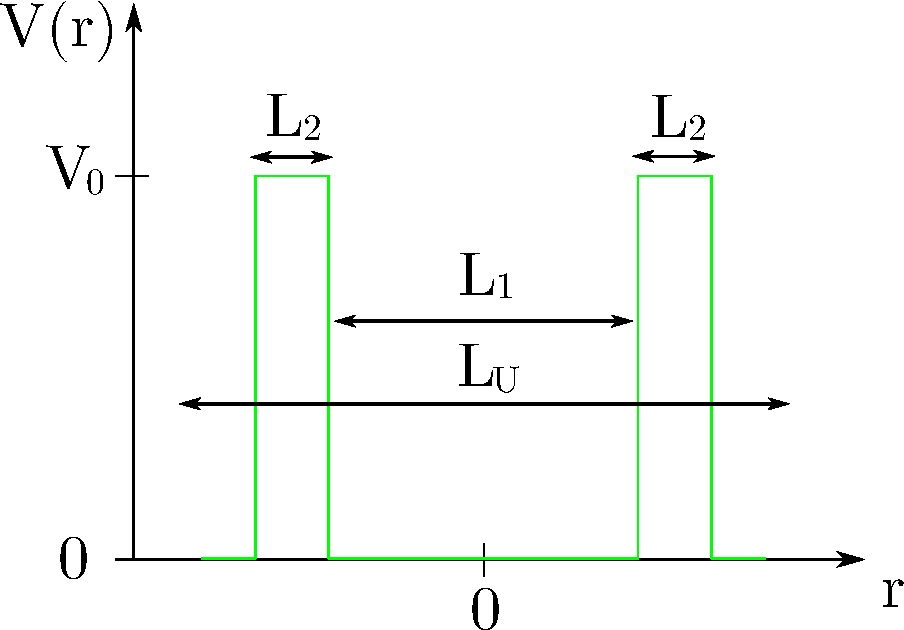
\includegraphics[width=0.7\textwidth]{plots/potential.pdf}
  \caption{Potentialverlauf der RTD.}
  \label{fig:pot1}
\end{figure}
Die eingezeichneten Längen wählen wir wie in (paper) zu
\begin{align}
  L_1 &= \SI{6}{\nano\meter}\\
  L_2 &= \SI{5}{\nano\meter}\\
  L_U &= \SI{30}{\nano\meter} \; .
\end{align}
Hierin ist $L_U$ die Länge, über der die Spannung $U$ abfällt. Auch hier lassen sich wieder zwei Fälle unterscheiden.
\begin{itemize}
  \item Der Gleichgewichtsfall $U=0$. Hier kann als Randbedingung auf beiden Seiten die Fermi-Dirac-Statistik \ref{eq:fd_statistic} angenommen werden.
  \item Der Nicht-Gleichgewichtsfall $U>0$. Hier sind lediglich die \emph{inflow}-Bedingungen für positive Geschwindigkeiten am linken- und negative Geschwindigkeiten am rechten Rand des Rechengebietes bekannt.
\end{itemize}

\section{Strom- und Ladungsträgerdichte}
Aus der Dichtematrix $\rho(r,q,t)$ in Schwerpunkt- und Relativkoordinaten lassen sich Strom- und Ladungsträgerdichte ableiten. Es gilt
\begin{align}
  j(r,t) &= \frac{\hbar}{m}\Im{\partial_q \rho(r,q,t)|_{q=0}} \\
  n(r,t) &= \Re{\rho(r,q,t)|_{q=0}} \; .
  \label{eq:dichte}
\end{align}

\section{Selbstkonsistentes Potential}
Das Potential in dem Liouville-Operator \eqref{eq:Liouville-Operator} setzt sich zusammen aus dem Hartree Potential $u(x,y,z)$ sowie dem Heterostuktur Potential $V_s(x,y,z)$.
\begin{align}
  V(\vb{x}) = u(\vb{x}) + V_s(\vb{x})
\end{align}
Das Hartree Potential ist mit der Elektronendichte $n(\vb{x})$ durch die Poisson-Gleichung \cite{frensley}
\begin{align}
  -\div \epsilon(\vb{x}) \grad u(\vb{x}) = e^2 (n(\vb{x}) - N_D(\vb{x})) \; ,
  \label{eq:poisson}
\end{align}
verknüpft, wobei $N_D(\vb{x})$ die ortsabhängige Dichte der Donatoren in der Heterostuktur und $\epsilon(\vb{x})$ die Permittivität bezeichnet.
Die Randbedingungen für $u$ ergeben sich aus der Forderung nach Ladungsneutralität in ausreichend großer Entfernung  \cite{frensley}
\begin{align}
  u|_{\partial\Omega} = \mu(\vb{x})|_{\partial\Omega}-V_s(\vb{x})|_{\partial\Omega}-\frac{1}{\beta}\mathcal{F}_{1/2}^{-1}(N_D/N_C) \; .
  \label{eq:RB_PE}
\end{align}
Hierin ist $\mu(\vb{x})$ das chemische Potential, $\beta=1/(k_BT)$ mit $T=\SI{300}{\kelvin}$, $N_C = 2(m^*/2\pi\hbar^2\beta)^{3/2}$ die "effektive Zustandsdichte" und $\mathcal{F}_{1/2}$ das Fermi-Dirac Integral der Ordnung $1/2$:
\begin{align}
  \mathcal{F}_j(x)=\frac{1}{\Gamma(j+1)}\int_0^{\infty}\frac{t^j}{\exp(t-x)+1}\diff t
\end{align}
Das Potential ergibt sich nach Gleichungen \eqref{eq:poisson} und \eqref{eq:dichte} aus dem Dichteoperator -- umgekehrt ergibt sich der Dichteoperator nach Gleichung \eqref{eq:lvn} aus dem Potential. Die Beziehung zwischen Potential und Dichte ist nicht-linear. Die gleichzeitige Lösung für Poisson- und \lvn zu finden erfordert daher Iteration. Das Problem wird \emph{selbstkonsistent} gelöst. Dazu löst man für $\eqref{eq:lvn}$ zunächst mit einem geeigneten \emph{initial guess} $V^{(0)}$. Nun wird iteriert und alternierend gelöst, bis Dichte und Potential sich nicht mehr signifikant ändern. Im Fall der transienten Betrachtung entspricht eine Iteration gleichzeitig einem Zeitschritt. Das Verfahren ist als \emph{Gummel (Plug-in) Approach} etabliert und beispielsweise in \cite{gummel} beschrieben. Die folgenden Ausführungen orientieren sich an dieser Literaturquelle.

Numerisch behandeln wir Gleichung \eqref{eq:poisson} mit dem Finite-Differenzen Verfahren. Das Rechengebiet $L$ wird diskretisiert gemäß
\begin{align}
  L_N \equiv \{x_i | x_i = i h \,\forall\, i = 0,1,\dots,N\text{ mit }L=Nh\}
\end{align}
Aus der Taylorentwicklung einer Funktion $f:L \rightarrow \mathbb{R}$ folgt für die Ableitungen
\begin{align}
  f'(x_i) &= \frac{f(x_{i+1}) - f(x_{i-1})}{2h} + \mathcal{O}(h^2) \\
  f''(x_i) &= \frac{f(x_{i+1}) - 2f(x_i) + f(x_{i-1})}{h^2} + \mathcal{O}(h^2) \; .
\end{align}
Wir schreiben kurz $f(x_i)\equiv f_i$.
Damit lässt sich mit $a_i\equiv (\epsilon_{i+1} - \epsilon_{i-1})/(4h^2\epsilon_i)$ Gleichung \eqref{eq:poisson} umschreiben zu
\begin{align}
  u_{i+1}\cdot(1+a_i) -2 u_i + u_{i-1}\cdot(1-a_i) - \underbrace{e^2h^2\frac{(N_{D,i} - n_i)}{\epsilon_i}}_{\equiv \text{rhs}_i} = 0\; ,
  \label{eq:discretePE}
\end{align}
wobei berücksichtigt werden muss, dass $u_0$ und $u_N$ über die Randbedingungen nach Gleichung \eqref{eq:RB_PE} vorgegeben sind. Somit haben wir das LGS
\begin{align}
  \left[ \begin{matrix}-2 & 1+a_1 & & & 0\\1-a_2 & \ddots & \ddots & & \\ & \ddots & \ddots & \ddots & \\& & \ddots & \ddots &  1+a_{N-2} \\0 & &  & 1-a_{N-1} & -2  \end{matrix}  \right]
  \left[ \begin{matrix}u_1             \\                          \\ \vdots                       \\                           \\u_{N-1}  \end{matrix}  \right]
  = \left[ \begin{matrix}\text{rhs}_1  \\                          \\ \vdots                       \\                         \\\text{rhs}_{N-1}  \end{matrix}  \right]
   - \left[ \begin{matrix}(1-a_1)u_0     \\0                         \\ \vdots                      \\0                        \\(1+a_{N-1})u_N  \end{matrix}  \right]
\end{align}
zu lösen. An dieser Stelle halten wir kurz inne und fragen uns, ob wir nicht eine "bessere" Vorhersage für $u^{(n+1)}$ treffen können, sodass wir eine schnellere Konvergenz der Iteration erreichen können. Diese Überlegung führt uns auf das verallgemeinerte Newton-Raphson-Verfahren.
Die linke Seite von Gleichung \eqref{eq:discretePE} definieren wir als Funktion $P_i(u_1,\dots,u_N)$ und wenden hierauf das Newton-Raphson-Verfahren an. Ausgehend von einem Startwert $\vb{u}^{(0)}$ erhalten wir das Fixpunktproblem
\begin{align}
  \vb{u}^{(n+1)} = \vb{u}^{(n)} - (\mathrm{D}\vb{P}|_{\vb{u}^{(n)}})^{-1} \vb{P}(\vb{u}^{(n)}) \; ,
  \label{eq:fixpunkt_gummel}
\end{align}
wobei wir die Vektorschreibweise
\begin{align}
  \vb{f} = \left( f_0,\dots,f_N\right)^T = \left( f(x_0),\dots,f(x_N)\right)^T
\end{align}
eingeführt haben und $\mathrm{D}$ der Differentiationsoperator ist, in diesem Fall also die Jacobik Matrix von $P$.
\begin{align}
  \left(\mathrm{D}\vb{P}|_{\vb{u}^{(n)}}\right)_{i,j} &= \pd{P_i}{u_j^{(n)}} \\ &\stackrel{\eqref{eq:discretePE}}{=}
  (1+a_i)\delta_{i+1,j} - 2 \delta_{i,j} + (1-a_i)\delta_{i-1,j} + \frac{e^2h^2}{\epsilon_i}\pd{n_i^{(n)}}{u_j^{(n)}}
\end{align}
An dieser Stelle ist anzumerken, dass nun auch die Dichte $n$ einen Iterationsindex $(n)$ bekommen hat. Dies ist auf die eingangs beschriebene alternierende Iteration zurückzuführen, in welcher abwechselnd $n^{(n)}$ und $u^{(n)}$ in einem einzigen Iterationsschritt $(n)$ berechnet werden. Ferner ist die Ableitung $\pd{n_i^{(n)}}{u_j^{(n)}}$ zunächst nicht bekannt.
Es ist überhaupt eine Abweichung $\pd{n_i^{(n)}}{u_j^{(n)}} \neq 0$, die den Unterschied zwischen Newton-Iteration und direktem Lösen bewirkt. Im Allgemeinen liegt keine exakte Form dieser Ableitung vor, da hierzu ja gerade die \lvn zu lösen ist. Es lässt sich jedoch eine Abschätzung vornehmen, welche schnell und kostengünstig ist, sodass das Newton-Verfahren einen echten Vorteil gegenüber dem direkten Iterieren hat. Dazu bedient man sich eines klassischen Gleichgewichts-Resultats und nimmt mit
\begin{align}
  n(u) = N_0\exp\left(\frac{u-u_0}{k_B T}\right)
  \label{eq:maxwell_boltzmann}
\end{align}
eine Maxwell-Boltzmann-Statistik an. Dies ist wohlgemerkt eine Annahme und es lassen sich ebenso andere Annehmen, z.B. eine Fermi-Dirac-Statistik, wählen. Jedoch zeigt sich in der Praxis, dass diese Wahl zuverlässig zu einer Konvergenz des Verfahrens führt. Falls nicht stationär, sondern transient gelöst werden soll, sollte jedoch das Newton-Verfahren nicht verwendet werden, da ein Iterationsschritt hier einem Zeitschritt entspricht und die Annahme \eqref{eq:maxwell_boltzmann} heuristischer Natur ist. Somit würde physikalisches Verhalten implizit aufgeprägt werden, statt dass dieses durch die vorhandenen zwei Gleichungen beschrieben wird.

Für den stationären Fall folgt aus Annahme \eqref{eq:maxwell_boltzmann} für das diskretisierte System
\begin{align}
  \pd{n_i}{u_j} = \frac{n_i}{k_B T}\delta_{i,j} \; .
\end{align}
Statt die Jacobi-Matrix invertieren zu müssen, schreiben wir Gleichung \eqref{eq:fixpunkt_gummel} um.
\begin{align}
  \mathrm{D}\vb{P}|_{\vb{u}^{(n)}}(\vb{u}^{(n+1)} - \vb{u}^{(n)}) = -  \vb{P}(\vb{u^{(n)}})
\end{align}
Explizit ausgeschrieben
\begin{align}
  \left(\mathrm{D}\vb{P}|_{\vb{u}^{(n)}}\right)_{i,j} &=
    (1+a_i)\delta_{i+1,j} + ( \frac{e^2h^2}{\epsilon_i}\frac{n_i}{k_B T} - 2) \delta_{i,j} + (1-a_i)\delta_{i-1,j} \\
  \left( \vb{P}(\vb{u^{(n)}}) \right)_{i} &=
   u_{i+1}^{(n)}\cdot(1+a_i) -2 u_i^{(n)} + u_{i-1}^{(n)}\cdot(1-a_i) - e^2h^2\frac{(N_{D,i} - n_i^{(n)})}{\epsilon_i}
\end{align}
mit $i,j = 1,\dots,N-1$. Wir lösen das LGS für $(\vb{u}^{(n+1)} - \vb{u}^{(n)})$ und erhalten
\begin{align}
  \vb{u}^{(n+1)} = (\vb{u}^{(n+1)} - \vb{u}^{(n)}) + \vb{u}^{(n)} \; .
\end{align}



\section{Wigner Funktion}
\label{sec:wignerfunktion}
Es ist mit $\bra{x}\ket{\Psi} = \Psi(x)$
\begin{equation}
  P(x,p) \equiv \frac{1}{\pi\hbar} \int_{-\infty}^{\infty} \bra{x+y}\hat{\rho} \ket{x-y} \E{2ipy/\hbar} \diff y
\end{equation}
die Wigner-Funktion gleich der Wigner-transformierten des Dichteoperators $\hat{\rho}$. Die Wigner Transformation ist eine invertierbare Abbildung
\begin{align}
  W\; :\; L(\HR,\HR)  \rightarrow & \text{Phasenraum}^* \\
   \hat{G} \mapsto & g(x,p) = \int_{-\infty}^{\infty} \bra{x-s/2}\hat{G} \ket{x+s/2} \E{ips/\hbar} \diff s
\end{align}
